\documentclass[]{article}
\usepackage{lmodern}
\usepackage{amssymb,amsmath}
\usepackage{ifxetex,ifluatex}
\usepackage{fixltx2e} % provides \textsubscript
\ifnum 0\ifxetex 1\fi\ifluatex 1\fi=0 % if pdftex
  \usepackage[T1]{fontenc}
  \usepackage[utf8]{inputenc}
\else % if luatex or xelatex
  \ifxetex
    \usepackage{mathspec}
  \else
    \usepackage{fontspec}
  \fi
  \defaultfontfeatures{Ligatures=TeX,Scale=MatchLowercase}
\fi
% use upquote if available, for straight quotes in verbatim environments
\IfFileExists{upquote.sty}{\usepackage{upquote}}{}
% use microtype if available
\IfFileExists{microtype.sty}{%
\usepackage{microtype}
\UseMicrotypeSet[protrusion]{basicmath} % disable protrusion for tt fonts
}{}
\usepackage[margin=1in]{geometry}
\usepackage{hyperref}
\hypersetup{unicode=true,
            pdftitle={Charactersing effect of anaemia on mortality in severe malaria},
            pdfborder={0 0 0},
            breaklinks=true}
\urlstyle{same}  % don't use monospace font for urls
\usepackage{color}
\usepackage{fancyvrb}
\newcommand{\VerbBar}{|}
\newcommand{\VERB}{\Verb[commandchars=\\\{\}]}
\DefineVerbatimEnvironment{Highlighting}{Verbatim}{commandchars=\\\{\}}
% Add ',fontsize=\small' for more characters per line
\usepackage{framed}
\definecolor{shadecolor}{RGB}{248,248,248}
\newenvironment{Shaded}{\begin{snugshade}}{\end{snugshade}}
\newcommand{\KeywordTok}[1]{\textcolor[rgb]{0.13,0.29,0.53}{\textbf{#1}}}
\newcommand{\DataTypeTok}[1]{\textcolor[rgb]{0.13,0.29,0.53}{#1}}
\newcommand{\DecValTok}[1]{\textcolor[rgb]{0.00,0.00,0.81}{#1}}
\newcommand{\BaseNTok}[1]{\textcolor[rgb]{0.00,0.00,0.81}{#1}}
\newcommand{\FloatTok}[1]{\textcolor[rgb]{0.00,0.00,0.81}{#1}}
\newcommand{\ConstantTok}[1]{\textcolor[rgb]{0.00,0.00,0.00}{#1}}
\newcommand{\CharTok}[1]{\textcolor[rgb]{0.31,0.60,0.02}{#1}}
\newcommand{\SpecialCharTok}[1]{\textcolor[rgb]{0.00,0.00,0.00}{#1}}
\newcommand{\StringTok}[1]{\textcolor[rgb]{0.31,0.60,0.02}{#1}}
\newcommand{\VerbatimStringTok}[1]{\textcolor[rgb]{0.31,0.60,0.02}{#1}}
\newcommand{\SpecialStringTok}[1]{\textcolor[rgb]{0.31,0.60,0.02}{#1}}
\newcommand{\ImportTok}[1]{#1}
\newcommand{\CommentTok}[1]{\textcolor[rgb]{0.56,0.35,0.01}{\textit{#1}}}
\newcommand{\DocumentationTok}[1]{\textcolor[rgb]{0.56,0.35,0.01}{\textbf{\textit{#1}}}}
\newcommand{\AnnotationTok}[1]{\textcolor[rgb]{0.56,0.35,0.01}{\textbf{\textit{#1}}}}
\newcommand{\CommentVarTok}[1]{\textcolor[rgb]{0.56,0.35,0.01}{\textbf{\textit{#1}}}}
\newcommand{\OtherTok}[1]{\textcolor[rgb]{0.56,0.35,0.01}{#1}}
\newcommand{\FunctionTok}[1]{\textcolor[rgb]{0.00,0.00,0.00}{#1}}
\newcommand{\VariableTok}[1]{\textcolor[rgb]{0.00,0.00,0.00}{#1}}
\newcommand{\ControlFlowTok}[1]{\textcolor[rgb]{0.13,0.29,0.53}{\textbf{#1}}}
\newcommand{\OperatorTok}[1]{\textcolor[rgb]{0.81,0.36,0.00}{\textbf{#1}}}
\newcommand{\BuiltInTok}[1]{#1}
\newcommand{\ExtensionTok}[1]{#1}
\newcommand{\PreprocessorTok}[1]{\textcolor[rgb]{0.56,0.35,0.01}{\textit{#1}}}
\newcommand{\AttributeTok}[1]{\textcolor[rgb]{0.77,0.63,0.00}{#1}}
\newcommand{\RegionMarkerTok}[1]{#1}
\newcommand{\InformationTok}[1]{\textcolor[rgb]{0.56,0.35,0.01}{\textbf{\textit{#1}}}}
\newcommand{\WarningTok}[1]{\textcolor[rgb]{0.56,0.35,0.01}{\textbf{\textit{#1}}}}
\newcommand{\AlertTok}[1]{\textcolor[rgb]{0.94,0.16,0.16}{#1}}
\newcommand{\ErrorTok}[1]{\textcolor[rgb]{0.64,0.00,0.00}{\textbf{#1}}}
\newcommand{\NormalTok}[1]{#1}
\usepackage{graphicx,grffile}
\makeatletter
\def\maxwidth{\ifdim\Gin@nat@width>\linewidth\linewidth\else\Gin@nat@width\fi}
\def\maxheight{\ifdim\Gin@nat@height>\textheight\textheight\else\Gin@nat@height\fi}
\makeatother
% Scale images if necessary, so that they will not overflow the page
% margins by default, and it is still possible to overwrite the defaults
% using explicit options in \includegraphics[width, height, ...]{}
\setkeys{Gin}{width=\maxwidth,height=\maxheight,keepaspectratio}
\IfFileExists{parskip.sty}{%
\usepackage{parskip}
}{% else
\setlength{\parindent}{0pt}
\setlength{\parskip}{6pt plus 2pt minus 1pt}
}
\setlength{\emergencystretch}{3em}  % prevent overfull lines
\providecommand{\tightlist}{%
  \setlength{\itemsep}{0pt}\setlength{\parskip}{0pt}}
\setcounter{secnumdepth}{0}
% Redefines (sub)paragraphs to behave more like sections
\ifx\paragraph\undefined\else
\let\oldparagraph\paragraph
\renewcommand{\paragraph}[1]{\oldparagraph{#1}\mbox{}}
\fi
\ifx\subparagraph\undefined\else
\let\oldsubparagraph\subparagraph
\renewcommand{\subparagraph}[1]{\oldsubparagraph{#1}\mbox{}}
\fi

%%% Use protect on footnotes to avoid problems with footnotes in titles
\let\rmarkdownfootnote\footnote%
\def\footnote{\protect\rmarkdownfootnote}

%%% Change title format to be more compact
\usepackage{titling}

% Create subtitle command for use in maketitle
\newcommand{\subtitle}[1]{
  \posttitle{
    \begin{center}\large#1\end{center}
    }
}

\setlength{\droptitle}{-2em}
  \title{Charactersing effect of anaemia on mortality in severe malaria}
  \pretitle{\vspace{\droptitle}\centering\huge}
  \posttitle{\par}
  \author{}
  \preauthor{}\postauthor{}
  \date{}
  \predate{}\postdate{}


\begin{document}
\maketitle

{
\setcounter{tocdepth}{2}
\tableofcontents
}
\section{Background}\label{background}

This looks at the severe malaria legacy dataset from MORU

\section{Imputation of missing
variables}\label{imputation-of-missing-variables}

Quite a lot of the important covariates are missing in the older
studies. We use linear regression to estimate these unknown variables:

\begin{itemize}
\tightlist
\item
  Mising base deficit is imputed using bicarbonate (if available) else
  using respiratory rate
\item
  Missing Blood urea nitrogen is imputed using creatinine
\end{itemize}

Impute base deficit from bicarbonate

\begin{Shaded}
\begin{Highlighting}[]
\NormalTok{BD_and_bicarbonate =}\StringTok{ }\OperatorTok{!}\KeywordTok{is.na}\NormalTok{(Leg_data}\OperatorTok{$}\NormalTok{BD) }\OperatorTok{&}\StringTok{ }\OperatorTok{!}\KeywordTok{is.na}\NormalTok{(Leg_data}\OperatorTok{$}\NormalTok{bicarbonate)}
\KeywordTok{print}\NormalTok{(}\KeywordTok{paste}\NormalTok{(}\StringTok{'We have '}\NormalTok{, }\KeywordTok{sum}\NormalTok{(BD_and_bicarbonate), }\StringTok{'observations for both bicarbonate and base deficit'}\NormalTok{))}
\end{Highlighting}
\end{Shaded}

\begin{verbatim}
## [1] "We have  5048 observations for both bicarbonate and base deficit"
\end{verbatim}

\begin{Shaded}
\begin{Highlighting}[]
\NormalTok{mod_impute1 =}\StringTok{ }\KeywordTok{lmer}\NormalTok{(BD }\OperatorTok{~}\StringTok{ }\NormalTok{bicarbonate }\OperatorTok{+}\StringTok{ }\NormalTok{(}\DecValTok{1} \OperatorTok{|}\StringTok{ }\NormalTok{studyID), }\DataTypeTok{data=}\NormalTok{ Leg_data[BD_and_bicarbonate,])}
\NormalTok{missing_BD =}\StringTok{ }\KeywordTok{is.na}\NormalTok{(Leg_data}\OperatorTok{$}\NormalTok{BD)}
\NormalTok{Available_Bicarbonate =}\StringTok{ }\OperatorTok{!}\KeywordTok{is.na}\NormalTok{(Leg_data}\OperatorTok{$}\NormalTok{bicarbonate)}
\KeywordTok{print}\NormalTok{(}\KeywordTok{paste}\NormalTok{(}\KeywordTok{sum}\NormalTok{(missing_BD }\OperatorTok{&}\StringTok{ }\NormalTok{Available_Bicarbonate), }\StringTok{'observations will now be imputed'}\NormalTok{))}
\end{Highlighting}
\end{Shaded}

\begin{verbatim}
## [1] "309 observations will now be imputed"
\end{verbatim}

\begin{Shaded}
\begin{Highlighting}[]
\CommentTok{# impute with model}
\NormalTok{Leg_data}\OperatorTok{$}\NormalTok{BD[missing_BD }\OperatorTok{&}\StringTok{ }\NormalTok{Available_Bicarbonate] =}\StringTok{ }\KeywordTok{predict}\NormalTok{(mod_impute1,}\DataTypeTok{newdata=}\NormalTok{Leg_data[missing_BD }\OperatorTok{&}\StringTok{ }\NormalTok{Available_Bicarbonate,], }\DataTypeTok{re.form=}\OtherTok{NA}\NormalTok{)}
\end{Highlighting}
\end{Shaded}

Impute base deficit from respiratory rate

\begin{Shaded}
\begin{Highlighting}[]
\NormalTok{BD_and_rr =}\StringTok{ }\OperatorTok{!}\KeywordTok{is.na}\NormalTok{(Leg_data}\OperatorTok{$}\NormalTok{BD) }\OperatorTok{&}\StringTok{ }\OperatorTok{!}\KeywordTok{is.na}\NormalTok{(Leg_data}\OperatorTok{$}\NormalTok{rr)}
\KeywordTok{print}\NormalTok{(}\KeywordTok{paste}\NormalTok{(}\StringTok{'We have '}\NormalTok{, }\KeywordTok{sum}\NormalTok{(BD_and_rr), }\StringTok{'observations for both resp rate and base deficit'}\NormalTok{))}
\end{Highlighting}
\end{Shaded}

\begin{verbatim}
## [1] "We have  6560 observations for both resp rate and base deficit"
\end{verbatim}

\begin{Shaded}
\begin{Highlighting}[]
\NormalTok{mod_impute2 =}\StringTok{ }\KeywordTok{lmer}\NormalTok{(BD }\OperatorTok{~}\StringTok{ }\NormalTok{rr }\OperatorTok{+}\StringTok{ }\NormalTok{(}\DecValTok{1} \OperatorTok{|}\StringTok{ }\NormalTok{studyID), }\DataTypeTok{data=}\NormalTok{ Leg_data[BD_and_rr,])}
\NormalTok{missing_BD =}\StringTok{ }\KeywordTok{is.na}\NormalTok{(Leg_data}\OperatorTok{$}\NormalTok{BD)}
\NormalTok{Available_rr =}\StringTok{ }\OperatorTok{!}\KeywordTok{is.na}\NormalTok{(Leg_data}\OperatorTok{$}\NormalTok{rr)}
\KeywordTok{print}\NormalTok{(}\KeywordTok{paste}\NormalTok{(}\KeywordTok{sum}\NormalTok{(missing_BD }\OperatorTok{&}\StringTok{ }\NormalTok{Available_rr), }\StringTok{'observations will now be imputed'}\NormalTok{))}
\end{Highlighting}
\end{Shaded}

\begin{verbatim}
## [1] "2662 observations will now be imputed"
\end{verbatim}

\begin{Shaded}
\begin{Highlighting}[]
\NormalTok{Leg_data}\OperatorTok{$}\NormalTok{BD[missing_BD }\OperatorTok{&}\StringTok{ }\NormalTok{Available_rr] =}\StringTok{ }\KeywordTok{predict}\NormalTok{(mod_impute2,}\DataTypeTok{newdata=}\NormalTok{Leg_data[missing_BD }\OperatorTok{&}\StringTok{ }\NormalTok{Available_rr,], }\DataTypeTok{re.form=}\OtherTok{NA}\NormalTok{)}
\end{Highlighting}
\end{Shaded}

Impute blood urea nitrogen from creatinine:

\begin{Shaded}
\begin{Highlighting}[]
\NormalTok{BUN_and_cr =}\StringTok{ }\OperatorTok{!}\KeywordTok{is.na}\NormalTok{(Leg_data}\OperatorTok{$}\NormalTok{BUN) }\OperatorTok{&}\StringTok{ }\OperatorTok{!}\KeywordTok{is.na}\NormalTok{(Leg_data}\OperatorTok{$}\NormalTok{creatinine)}
\KeywordTok{print}\NormalTok{(}\KeywordTok{paste}\NormalTok{(}\StringTok{'We have '}\NormalTok{, }\KeywordTok{sum}\NormalTok{(BUN_and_cr), }\StringTok{'observations for both blood urea nitrogen and creatinine'}\NormalTok{))}
\end{Highlighting}
\end{Shaded}

\begin{verbatim}
## [1] "We have  1433 observations for both blood urea nitrogen and creatinine"
\end{verbatim}

\begin{Shaded}
\begin{Highlighting}[]
\NormalTok{mod_impute3 =}\StringTok{ }\KeywordTok{lmer}\NormalTok{(BUN }\OperatorTok{~}\StringTok{ }\NormalTok{creatinine }\OperatorTok{+}\StringTok{ }\NormalTok{(}\DecValTok{1} \OperatorTok{|}\StringTok{ }\NormalTok{studyID), }\DataTypeTok{data=}\NormalTok{ Leg_data[BUN_and_cr,])}
\NormalTok{missing_BUN =}\StringTok{ }\KeywordTok{is.na}\NormalTok{(Leg_data}\OperatorTok{$}\NormalTok{BUN)}
\NormalTok{Available_cr =}\StringTok{ }\OperatorTok{!}\KeywordTok{is.na}\NormalTok{(Leg_data}\OperatorTok{$}\NormalTok{creatinine)}
\KeywordTok{print}\NormalTok{(}\KeywordTok{paste}\NormalTok{(}\KeywordTok{sum}\NormalTok{(missing_BUN }\OperatorTok{&}\StringTok{ }\NormalTok{Available_cr), }\StringTok{'observations will now be imputed'}\NormalTok{))}
\end{Highlighting}
\end{Shaded}

\begin{verbatim}
## [1] "679 observations will now be imputed"
\end{verbatim}

\begin{Shaded}
\begin{Highlighting}[]
\NormalTok{Leg_data}\OperatorTok{$}\NormalTok{BUN[missing_BUN }\OperatorTok{&}\StringTok{ }\NormalTok{Available_cr] =}\StringTok{ }\KeywordTok{predict}\NormalTok{(mod_impute3,}\DataTypeTok{newdata=}\NormalTok{Leg_data[missing_BUN }\OperatorTok{&}\StringTok{ }\NormalTok{Available_cr,], }\DataTypeTok{re.form=}\OtherTok{NA}\NormalTok{)}
\end{Highlighting}
\end{Shaded}

Resulting data we can now use: The contributions of the different
studies:

\begin{Shaded}
\begin{Highlighting}[]
\NormalTok{vars_interest =}\StringTok{ }\KeywordTok{c}\NormalTok{(}\StringTok{'outcome'}\NormalTok{,}\StringTok{'HCT'}\NormalTok{,}\StringTok{'LPAR_pct'}\NormalTok{,}\StringTok{'BD'}\NormalTok{,}\StringTok{'BUN'}\NormalTok{,}\StringTok{'poedema'}\NormalTok{,}\StringTok{'convulsions'}\NormalTok{,}\StringTok{'coma'}\NormalTok{,}\StringTok{'AgeInYear'}\NormalTok{,}\StringTok{'drug_class'}\NormalTok{)}
\NormalTok{complete_cases =}\StringTok{ }\KeywordTok{apply}\NormalTok{(Leg_data[,vars_interest], }\DecValTok{1}\NormalTok{, }\ControlFlowTok{function}\NormalTok{(x) }\KeywordTok{sum}\NormalTok{(}\KeywordTok{is.na}\NormalTok{(x))) }\OperatorTok{==}\StringTok{ }\DecValTok{0}
\NormalTok{Complete_Leg_data =}\StringTok{ }\NormalTok{Leg_data[complete_cases,] }\CommentTok{# for the model fitting}
\NormalTok{Complete_Leg_data}\OperatorTok{$}\NormalTok{studyID =}\StringTok{ }\KeywordTok{as.factor}\NormalTok{(}\KeywordTok{as.character}\NormalTok{(Complete_Leg_data}\OperatorTok{$}\NormalTok{studyID))}
\CommentTok{# Whole dataset}
\KeywordTok{table}\NormalTok{(Leg_data}\OperatorTok{$}\NormalTok{studyID)}
\end{Highlighting}
\end{Shaded}

\begin{verbatim}
## 
##          AAV           AQ     AQGambia      AQUAMAT Core Malaria 
##          370          560          579         5494         1121 
##    SEAQUAMAT 
##         1461
\end{verbatim}

\begin{Shaded}
\begin{Highlighting}[]
\CommentTok{# in the complete dataset (all variables recorded)}
\KeywordTok{table}\NormalTok{(Complete_Leg_data}\OperatorTok{$}\NormalTok{studyID)}
\end{Highlighting}
\end{Shaded}

\begin{verbatim}
## 
##          AAV           AQ     AQGambia      AQUAMAT Core Malaria 
##          213          150          168         3666          639 
##    SEAQUAMAT 
##         1333
\end{verbatim}

\begin{Shaded}
\begin{Highlighting}[]
\NormalTok{Complete_Leg_data}\OperatorTok{$}\NormalTok{drug_AS =}\StringTok{ }\DecValTok{0}
\NormalTok{Complete_Leg_data}\OperatorTok{$}\NormalTok{drug_AS[Complete_Leg_data}\OperatorTok{$}\NormalTok{drug_class}\OperatorTok{==}\StringTok{'artemisinin'}\NormalTok{]=}\DecValTok{1}

\CommentTok{# remove infinite log parasitaemias}
\NormalTok{ind_keep =}\StringTok{ }\OperatorTok{!}\NormalTok{(}\KeywordTok{is.infinite}\NormalTok{(Complete_Leg_data}\OperatorTok{$}\NormalTok{LPAR_pct) }\OperatorTok{|}\StringTok{ }\KeywordTok{is.nan}\NormalTok{(Complete_Leg_data}\OperatorTok{$}\NormalTok{LPAR_pct))}
\NormalTok{Complete_Leg_data =}\StringTok{ }\NormalTok{Complete_Leg_data[ind_keep,]}
\end{Highlighting}
\end{Shaded}

\section{Exploratory analysis}\label{exploratory-analysis}

Let's look at the key predictive variables. We use a random effects term
to model differences between studies.
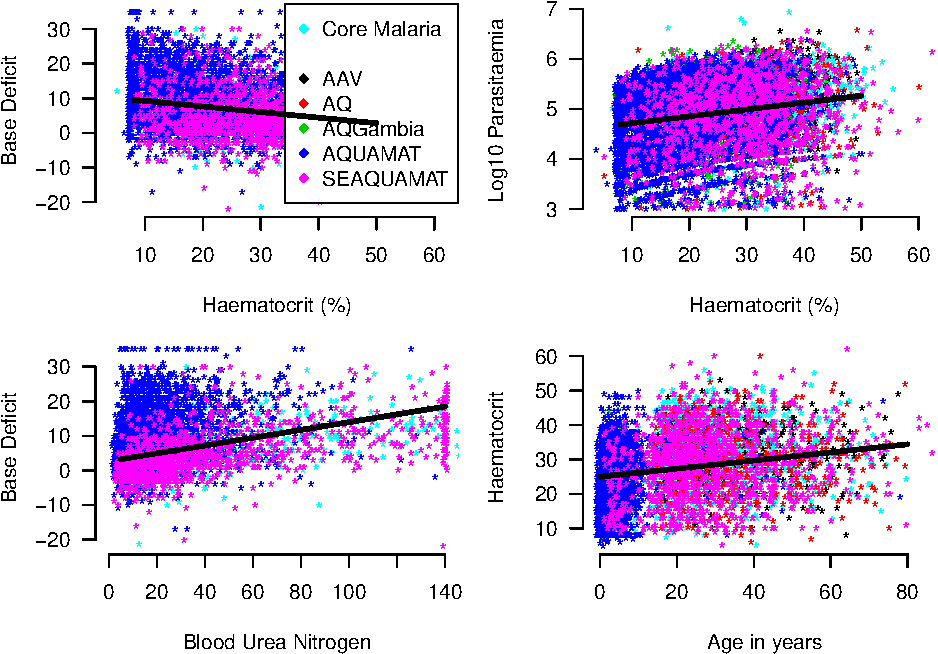
\includegraphics{LegacyAnalysis_files/figure-latex/ExploratoryPlots-1.pdf}

\section{Predictive value of anaemia on death adjusting for
confounders}\label{predictive-value-of-anaemia-on-death-adjusting-for-confounders}

Before fitting the more complex GAM models we explore the standard glm
(logistic regression) models.

\begin{Shaded}
\begin{Highlighting}[]
\NormalTok{mod_full =}\StringTok{ }\KeywordTok{glmer}\NormalTok{(outcome }\OperatorTok{~}\StringTok{ }\NormalTok{HCT }\OperatorTok{+}\StringTok{ }\NormalTok{LPAR_pct }\OperatorTok{+}\StringTok{ }\NormalTok{AgeInYear }\OperatorTok{+}\StringTok{ }\NormalTok{coma }\OperatorTok{+}\StringTok{ }\NormalTok{convulsions }\OperatorTok{+}
\StringTok{                   }\NormalTok{poedema }\OperatorTok{+}\StringTok{ }\NormalTok{BUN }\OperatorTok{+}\StringTok{ }\NormalTok{BD }\OperatorTok{+}\StringTok{ }\NormalTok{drug_AS }\OperatorTok{+}\StringTok{ }\NormalTok{(}\DecValTok{1} \OperatorTok{|}\StringTok{ }\NormalTok{studyID),}
               \DataTypeTok{data=}\NormalTok{Complete_Leg_data, }\DataTypeTok{family=}\NormalTok{binomial)}
\end{Highlighting}
\end{Shaded}

\begin{verbatim}
## Warning in checkConv(attr(opt, "derivs"), opt$par, ctrl = control$checkConv, : Model is nearly unidentifiable: very large eigenvalue
##  - Rescale variables?
\end{verbatim}

\begin{Shaded}
\begin{Highlighting}[]
\KeywordTok{summary}\NormalTok{(mod_full)}
\end{Highlighting}
\end{Shaded}

\begin{verbatim}
## Generalized linear mixed model fit by maximum likelihood (Laplace
##   Approximation) [glmerMod]
##  Family: binomial  ( logit )
## Formula: 
## outcome ~ HCT + LPAR_pct + AgeInYear + coma + convulsions + poedema +  
##     BUN + BD + drug_AS + (1 | studyID)
##    Data: Complete_Leg_data
## 
##      AIC      BIC   logLik deviance df.resid 
##   3550.0   3623.9  -1764.0   3528.0     6086 
## 
## Scaled residuals: 
##     Min      1Q  Median      3Q     Max 
## -5.7815 -0.3459 -0.2035 -0.1263 11.0067 
## 
## Random effects:
##  Groups  Name        Variance Std.Dev.
##  studyID (Intercept) 0.02104  0.1451  
## Number of obs: 6097, groups:  studyID, 6
## 
## Fixed effects:
##               Estimate Std. Error z value Pr(>|z|)    
## (Intercept)  -4.948185   0.213543 -23.172  < 2e-16 ***
## HCT           0.014758   0.005204   2.836 0.004571 ** 
## LPAR_pct      0.055263   0.060015   0.921 0.357144    
## AgeInYear     0.019206   0.003808   5.044 4.56e-07 ***
## coma          1.413142   0.097127  14.549  < 2e-16 ***
## convulsions1  0.466693   0.111460   4.187 2.83e-05 ***
## poedema1      0.778130   0.371496   2.095 0.036208 *  
## BUN           0.013336   0.001544   8.637  < 2e-16 ***
## BD            0.129810   0.007001  18.543  < 2e-16 ***
## drug_AS      -0.322689   0.089086  -3.622 0.000292 ***
## ---
## Signif. codes:  0 '***' 0.001 '**' 0.01 '*' 0.05 '.' 0.1 ' ' 1
## 
## Correlation of Fixed Effects:
##             (Intr) HCT    LPAR_p AgInYr coma   cnvls1 poedm1 BUN    BD    
## HCT         -0.661                                                        
## LPAR_pct    -0.100  0.011                                                 
## AgeInYear   -0.250 -0.117 -0.057                                          
## coma        -0.246 -0.064  0.062 -0.068                                   
## convulsins1 -0.051 -0.075  0.035  0.101 -0.245                            
## poedema1    -0.013 -0.004 -0.004 -0.086  0.012  0.005                     
## BUN         -0.229  0.109 -0.055 -0.154  0.005  0.048 -0.020              
## BD          -0.428  0.223 -0.170  0.159  0.001  0.065  0.022 -0.207       
## drug_AS     -0.167 -0.009 -0.017 -0.069 -0.006  0.001 -0.023 -0.049 -0.013
## convergence code: 0
## Model is nearly unidentifiable: very large eigenvalue
##  - Rescale variables?
\end{verbatim}

Now let's make counterfactual predictions of anaemia on death for the
patients in the database.

\begin{Shaded}
\begin{Highlighting}[]
\NormalTok{myquantiles =}\StringTok{ }\KeywordTok{c}\NormalTok{(}\FloatTok{0.25}\NormalTok{,}\FloatTok{0.5}\NormalTok{,}\FloatTok{0.75}\NormalTok{) }\CommentTok{# this is 50% predictive interval}

\NormalTok{overall_median_mortality =}\StringTok{ }\KeywordTok{median}\NormalTok{(}\DecValTok{100}\OperatorTok{*}\KeywordTok{predict}\NormalTok{(mod_full, }\DataTypeTok{type=}\StringTok{'response'}\NormalTok{))}
\KeywordTok{par}\NormalTok{(}\DataTypeTok{las=}\DecValTok{1}\NormalTok{, }\DataTypeTok{bty=}\StringTok{'n'}\NormalTok{)}
\NormalTok{x_hcts =}\StringTok{ }\KeywordTok{seq}\NormalTok{(}\DecValTok{4}\NormalTok{,}\DecValTok{45}\NormalTok{, }\DataTypeTok{by=}\DecValTok{1}\NormalTok{)}
\NormalTok{probs_lin =}\StringTok{ }\KeywordTok{array}\NormalTok{(}\DataTypeTok{dim =} \KeywordTok{c}\NormalTok{(}\DecValTok{3}\NormalTok{, }\KeywordTok{length}\NormalTok{(x_hcts)))}
\ControlFlowTok{for}\NormalTok{(i }\ControlFlowTok{in} \DecValTok{1}\OperatorTok{:}\KeywordTok{length}\NormalTok{(x_hcts))\{}
\NormalTok{  mydata =}\StringTok{ }\NormalTok{Complete_Leg_data}
\NormalTok{  mydata}\OperatorTok{$}\NormalTok{HCT=x_hcts[i]}
\NormalTok{  ys =}\StringTok{ }\DecValTok{100}\OperatorTok{*}\KeywordTok{predict}\NormalTok{(mod_full, }\DataTypeTok{newdata =}\NormalTok{ mydata, }\DataTypeTok{re.form=}\OtherTok{NA}\NormalTok{, }\DataTypeTok{type=}\StringTok{'response'}\NormalTok{)}
\NormalTok{  probs_lin[,i] =}\StringTok{ }\KeywordTok{quantile}\NormalTok{(ys, }\DataTypeTok{probs=}\NormalTok{myquantiles)}
\NormalTok{\}}
\end{Highlighting}
\end{Shaded}

The way to interpret this `counterfactual' plot is as follows: suppose
that every individual in the dataset was assigned (as in a intervention)
a specific haematocrit \(X\), what would the resulting per patient
probability of death be. Here we summarise these probabilities by the
predicted mean probability of death and 80\% predictive intervals.

\begin{Shaded}
\begin{Highlighting}[]
\KeywordTok{plot}\NormalTok{(x_hcts,probs_lin[}\DecValTok{2}\NormalTok{,], }\DataTypeTok{xlim=}\KeywordTok{c}\NormalTok{(}\DecValTok{4}\NormalTok{,}\DecValTok{45}\NormalTok{), }\DataTypeTok{ylab=}\StringTok{'Predicted probability of death'}\NormalTok{, }
     \DataTypeTok{xlab=}\StringTok{'Haematocrit (%)'}\NormalTok{, }\DataTypeTok{ylim=}\KeywordTok{c}\NormalTok{(}\DecValTok{0}\NormalTok{,}\DecValTok{30}\NormalTok{), }\DataTypeTok{lty=}\DecValTok{1}\NormalTok{, }\DataTypeTok{lwd=}\DecValTok{3}\NormalTok{, }\DataTypeTok{type=}\StringTok{'l'}\NormalTok{)}
\KeywordTok{lines}\NormalTok{(x_hcts, probs_lin[}\DecValTok{1}\NormalTok{,], }\DataTypeTok{lty=}\DecValTok{2}\NormalTok{, }\DataTypeTok{lwd=}\DecValTok{2}\NormalTok{)}
\KeywordTok{lines}\NormalTok{(x_hcts, probs_lin[}\DecValTok{3}\NormalTok{,], }\DataTypeTok{lty=}\DecValTok{2}\NormalTok{, }\DataTypeTok{lwd=}\DecValTok{2}\NormalTok{)}
\KeywordTok{abline}\NormalTok{(}\DataTypeTok{h=}\NormalTok{overall_median_mortality, }\DataTypeTok{lwd=}\DecValTok{3}\NormalTok{, }\DataTypeTok{col=}\StringTok{'blue'}\NormalTok{,}\DataTypeTok{lty=}\DecValTok{2}\NormalTok{)}
\KeywordTok{legend}\NormalTok{(}\StringTok{'topleft'}\NormalTok{, }\DataTypeTok{col=}\KeywordTok{c}\NormalTok{(}\StringTok{'black'}\NormalTok{,}\StringTok{'black'}\NormalTok{,}\StringTok{'blue'}\NormalTok{), }\DataTypeTok{lwd=}\DecValTok{3}\NormalTok{, }\DataTypeTok{lty=}\KeywordTok{c}\NormalTok{(}\DecValTok{1}\NormalTok{,}\DecValTok{2}\NormalTok{,}\DecValTok{2}\NormalTok{),}
       \DataTypeTok{legend =} \KeywordTok{c}\NormalTok{(}\StringTok{'Median counterfactual value'}\NormalTok{, }\StringTok{'25th and 75th counterfactual quantiles'}\NormalTok{,}\StringTok{'Retrodicted median value'}\NormalTok{))}
\end{Highlighting}
\end{Shaded}

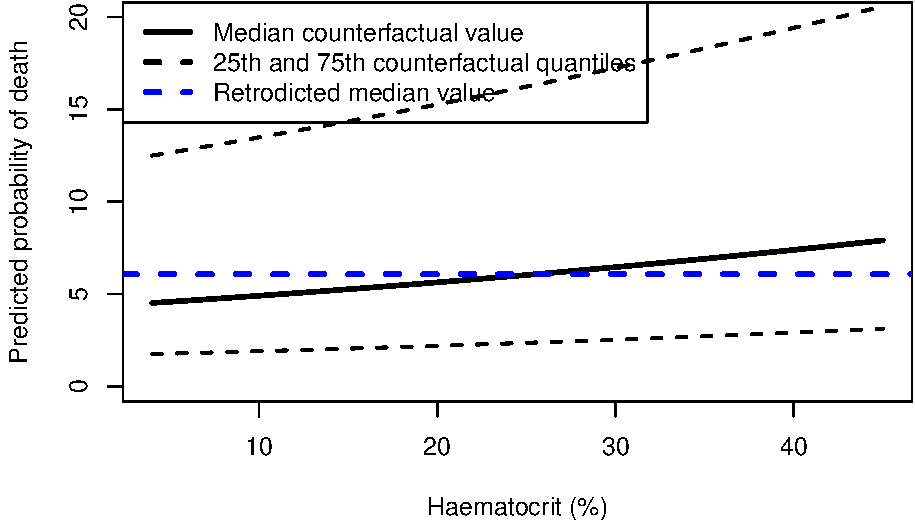
\includegraphics{LegacyAnalysis_files/figure-latex/unnamed-chunk-7-1.pdf}

\subsection{More complex GAM model}\label{more-complex-gam-model}

The GAM model allows for non-linear relationships between certain
variables and the outcome.

Here we fit as non-linear the effect of age and haematocrit on
mortality.

\begin{Shaded}
\begin{Highlighting}[]
\NormalTok{mod_full_GAM =}\StringTok{ }\KeywordTok{gam}\NormalTok{(outcome }\OperatorTok{~}\StringTok{ }\KeywordTok{s}\NormalTok{(HCT,AgeInYear) }\OperatorTok{+}\StringTok{ }\NormalTok{LPAR_pct  }\OperatorTok{+}\StringTok{ }\NormalTok{coma }\OperatorTok{+}\StringTok{ }\NormalTok{convulsions }\OperatorTok{+}
\StringTok{                   }\NormalTok{poedema }\OperatorTok{+}\StringTok{ }\NormalTok{BUN }\OperatorTok{+}\StringTok{ }\NormalTok{BD }\OperatorTok{+}\StringTok{ }\NormalTok{drug_AS,}
               \DataTypeTok{data=}\NormalTok{Complete_Leg_data, }\DataTypeTok{family=}\NormalTok{binomial)}
\KeywordTok{summary}\NormalTok{(mod_full_GAM)}
\end{Highlighting}
\end{Shaded}

\begin{verbatim}
## 
## Family: binomial 
## Link function: logit 
## 
## Formula:
## outcome ~ s(HCT, AgeInYear) + LPAR_pct + coma + convulsions + 
##     poedema + BUN + BD + drug_AS
## 
## Parametric coefficients:
##               Estimate Std. Error z value Pr(>|z|)    
## (Intercept)  -4.366081   0.125023 -34.922  < 2e-16 ***
## LPAR_pct      0.051699   0.058816   0.879 0.379400    
## coma          1.390986   0.096050  14.482  < 2e-16 ***
## convulsions1  0.511948   0.111127   4.607 4.09e-06 ***
## poedema1      0.738046   0.362458   2.036 0.041728 *  
## BUN           0.012307   0.001564   7.870 3.54e-15 ***
## BD            0.134255   0.007255  18.505  < 2e-16 ***
## drug_AS      -0.334316   0.088449  -3.780 0.000157 ***
## ---
## Signif. codes:  0 '***' 0.001 '**' 0.01 '*' 0.05 '.' 0.1 ' ' 1
## 
## Approximate significance of smooth terms:
##                    edf Ref.df Chi.sq p-value    
## s(HCT,AgeInYear) 7.006  9.781    102  <2e-16 ***
## ---
## Signif. codes:  0 '***' 0.001 '**' 0.01 '*' 0.05 '.' 0.1 ' ' 1
## 
## R-sq.(adj) =   0.25   Deviance explained = 26.5%
## UBRE = -0.4204  Scale est. = 1         n = 6097
\end{verbatim}

Now we compute the corresponding counterfactual probabilities of death
for the dataset for all values of the haematocrit:

\begin{Shaded}
\begin{Highlighting}[]
\NormalTok{overall_median_mortalityGAM =}\StringTok{ }\KeywordTok{median}\NormalTok{(}\DecValTok{100}\OperatorTok{*}\KeywordTok{predict}\NormalTok{(mod_full_GAM, }\DataTypeTok{type=}\StringTok{'response'}\NormalTok{))}
\KeywordTok{par}\NormalTok{(}\DataTypeTok{las=}\DecValTok{1}\NormalTok{, }\DataTypeTok{bty=}\StringTok{'n'}\NormalTok{)}
\NormalTok{probs_gam =}\StringTok{ }\KeywordTok{array}\NormalTok{(}\DataTypeTok{dim =} \KeywordTok{c}\NormalTok{(}\DecValTok{3}\NormalTok{, }\KeywordTok{length}\NormalTok{(x_hcts)))}
\ControlFlowTok{for}\NormalTok{(i }\ControlFlowTok{in} \DecValTok{1}\OperatorTok{:}\KeywordTok{length}\NormalTok{(x_hcts))\{}
\NormalTok{  mydata =}\StringTok{ }\NormalTok{Complete_Leg_data}
\NormalTok{  mydata}\OperatorTok{$}\NormalTok{HCT=x_hcts[i]}
\NormalTok{  ys =}\StringTok{ }\DecValTok{100}\OperatorTok{*}\KeywordTok{predict}\NormalTok{(mod_full_GAM, }\DataTypeTok{newdata =}\NormalTok{ mydata, }\DataTypeTok{re.form=}\OtherTok{NA}\NormalTok{, }\DataTypeTok{type=}\StringTok{'response'}\NormalTok{)}
\NormalTok{  probs_gam[,i] =}\StringTok{ }\KeywordTok{quantile}\NormalTok{(ys, }\DataTypeTok{probs=}\NormalTok{myquantiles)}
\NormalTok{\}}
\end{Highlighting}
\end{Shaded}

We see that the effect of haematocrit on mortality is non-linear under
this model: below 20 is protective, above 20 plateaus out:

\begin{Shaded}
\begin{Highlighting}[]
\CommentTok{#}
\KeywordTok{par}\NormalTok{(}\DataTypeTok{las=}\DecValTok{1}\NormalTok{, }\DataTypeTok{mfrow=}\KeywordTok{c}\NormalTok{(}\DecValTok{1}\NormalTok{,}\DecValTok{2}\NormalTok{), }\DataTypeTok{bty=}\StringTok{'n'}\NormalTok{, }\DataTypeTok{mar=}\KeywordTok{c}\NormalTok{(}\DecValTok{4}\NormalTok{,}\DecValTok{4}\NormalTok{,}\DecValTok{1}\NormalTok{,}\DecValTok{1}\NormalTok{))}
\NormalTok{### Plot the standard logistic regression model}
\KeywordTok{plot}\NormalTok{(x_hcts,probs_lin[}\DecValTok{2}\NormalTok{,], }\DataTypeTok{xlim=}\KeywordTok{c}\NormalTok{(}\DecValTok{4}\NormalTok{,}\DecValTok{45}\NormalTok{), }\DataTypeTok{ylab=}\StringTok{'Predicted probability of death'}\NormalTok{, }
     \DataTypeTok{xlab=}\StringTok{'Haematocrit (%)'}\NormalTok{, }\DataTypeTok{ylim=}\KeywordTok{c}\NormalTok{(}\DecValTok{0}\NormalTok{,}\DecValTok{20}\NormalTok{), }\DataTypeTok{lty=}\DecValTok{1}\NormalTok{, }\DataTypeTok{lwd=}\DecValTok{3}\NormalTok{, }\DataTypeTok{type=}\StringTok{'l'}\NormalTok{)}
\KeywordTok{lines}\NormalTok{(x_hcts, probs_lin[}\DecValTok{1}\NormalTok{,], }\DataTypeTok{lty=}\DecValTok{2}\NormalTok{, }\DataTypeTok{lwd=}\DecValTok{2}\NormalTok{)}
\KeywordTok{lines}\NormalTok{(x_hcts, probs_lin[}\DecValTok{3}\NormalTok{,], }\DataTypeTok{lty=}\DecValTok{2}\NormalTok{, }\DataTypeTok{lwd=}\DecValTok{2}\NormalTok{)}
\KeywordTok{abline}\NormalTok{(}\DataTypeTok{h=}\NormalTok{overall_median_mortality, }\DataTypeTok{lwd=}\DecValTok{3}\NormalTok{, }\DataTypeTok{col=}\StringTok{'blue'}\NormalTok{,}\DataTypeTok{lty=}\DecValTok{2}\NormalTok{)}
\KeywordTok{title}\NormalTok{(}\StringTok{'Logistic regression model'}\NormalTok{)}
\NormalTok{### And now the GAM model}
\KeywordTok{plot}\NormalTok{(x_hcts,probs_gam[}\DecValTok{2}\NormalTok{,], }\DataTypeTok{xlim=}\KeywordTok{c}\NormalTok{(}\DecValTok{4}\NormalTok{,}\DecValTok{45}\NormalTok{), }\DataTypeTok{ylab=}\StringTok{'Predicted probability of death'}\NormalTok{, }
     \DataTypeTok{xlab=}\StringTok{'Haematocrit (%)'}\NormalTok{, }\DataTypeTok{ylim=}\KeywordTok{c}\NormalTok{(}\DecValTok{0}\NormalTok{,}\DecValTok{20}\NormalTok{), }\DataTypeTok{lty=}\DecValTok{1}\NormalTok{, }\DataTypeTok{lwd=}\DecValTok{3}\NormalTok{, }\DataTypeTok{type=}\StringTok{'l'}\NormalTok{)}
\KeywordTok{lines}\NormalTok{(x_hcts, probs_gam[}\DecValTok{1}\NormalTok{,], }\DataTypeTok{lty=}\DecValTok{2}\NormalTok{, }\DataTypeTok{lwd=}\DecValTok{2}\NormalTok{)}
\KeywordTok{lines}\NormalTok{(x_hcts, probs_gam[}\DecValTok{3}\NormalTok{,], }\DataTypeTok{lty=}\DecValTok{2}\NormalTok{, }\DataTypeTok{lwd=}\DecValTok{2}\NormalTok{)}
\KeywordTok{abline}\NormalTok{(}\DataTypeTok{h=}\NormalTok{overall_median_mortalityGAM, }\DataTypeTok{lwd=}\DecValTok{3}\NormalTok{, }\DataTypeTok{col=}\StringTok{'blue'}\NormalTok{,}\DataTypeTok{lty=}\DecValTok{2}\NormalTok{)}
\KeywordTok{title}\NormalTok{(}\StringTok{'Generalised additive model'}\NormalTok{)}
\end{Highlighting}
\end{Shaded}

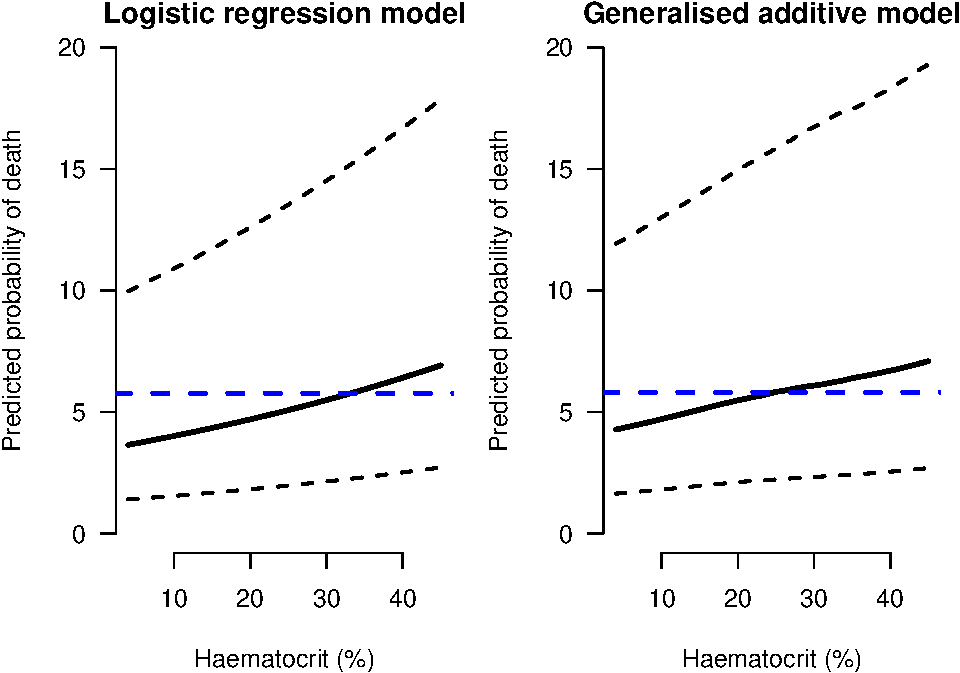
\includegraphics{LegacyAnalysis_files/figure-latex/counterfactualPlots-1.pdf}


\end{document}
